\documentclass[a4paper,twocolumn]{article} % Document type

\ifx\pdfoutput\undefined
    %Use old Latex if PDFLatex does not work
   \usepackage[dvips]{graphicx}% To get graphics working
   \DeclareGraphicsExtensions{.eps} % Encapsulated PostScript
 \else
    %Use PDFLatex
   \usepackage[pdftex]{graphicx}% To get graphics working
   \DeclareGraphicsExtensions{.pdf,.jpg,.png,.mps} % Portable Document Format, Joint Photographic Experts Group, Portable Network Graphics, MetaPost
   \pdfcompresslevel=9
\fi

\usepackage{amsmath,amssymb}   % Contains mathematical symbols
\usepackage[ansinew]{inputenc} % Input encoding, identical to Windows 1252
\usepackage[english]{babel}    % Language
%\usepackage[round,authoryear]{natbib}  %Nice author (year) citations
\usepackage[square,numbers]{natbib}     %Nice numbered citations
%\bibliographystyle{unsrtnat}           %Unsorted bibliography
\bibliographystyle{plainnat}            %Sorted bibliography

\addtolength{\topmargin}{-30mm}% Removes 30mm from the top margin
\addtolength{\textheight}{30mm}% Adds it to the text height


\begin{document}               % Begins the document

\title{Homework 1 in EL2620 Nonlinear Control}
\author{Yuchao Li \\ 910928-4233 \\ yuchao@kth.se \and Anqing Duan\\
  person number \\ email}
%\date{2010-10-10}             % If you want to set the date yourself.

\maketitle                     % Generates the title




%%%%%%%%%%%%%%%%%%%%%%%%%%%%%%%%%%%%%%%%%%%%%%%%%%%%%%%%%%%%%%%%%%%%%%%%%%%%%%%%%%%
% Instructions regarding the report
%%%%%%%%%%%%%%%%%%%%%%%%%%%%%%%%%%%%%%%%%%%%%%%%%%%%%%%%%%%%%%%%%%%%%%%%%%%%%%%%%%%

\section*{Problem description}
\label{sec:prob}

The change in population of two interacting species inhabiting a grassy island can be described by the following equations:
\begin{equation}\label{eqn:Model}
\begin{aligned} 
\dot{x}&=x(t)(a+bx(t)+cy(t)) \\
\dot{y}&=y(t)(d+ex(t)+fy(t))
\end{aligned}
\end{equation}
where $a, b, ... ,f$ are parameters and $x, y$ are non-negative continuous function with respect to time. First, the model can be effective only with two preconditions fulfilled. Second, the populations here are normalized and therefore can be thought of as continuous numbers. The habitat is isolated area, which means the impact from other creatures can be neglected. While $a, b, d$ and $f$ are very much dependent on food supply and intraspecific competition, $c$ and $e$ reflect biological interactions between those two species. This work seeks to provide more details of this model by analyzing the solutions of \eqref{eqn:Model} and their biological backgrounds when those constants are assigned with different numbers. A generalized model for more species is presented in the end.

%%%%%%%%%%%%%%%%%%%%%%%%%%%%%%%%%%%%%%%%%%%%%%%%%%%%%%%%%%%%%%%%%%%%%%%%%%%%%%%%%%%
% Example 1
%%%%%%%%%%%%%%%%%%%%%%%%%%%%%%%%%%%%%%%%%%%%%%%%%%%%%%%%%%%%%%%%%%%%%%%%%%%%%%%%%%%

\section*{Problem 1 -- Analysis of biological interaction}
\label{sec:pro1}

The relation between $x$ and $y$ can be interpreted in four different ways. It can be predator-prey ($x$ predator, $y$ prey), prey-predator ($x$ prey, $y$ predator), competitive ($x$ and $y$ inhibit each other) or symbiotic ($x$ and $y$ benefit each other). The sign of $c$ and $e$ defines the relation. The following solution elaborates the dependence.    

\section*{Solution 1 -- Analysis of biological interaction}
\label{sec:sol1}

\begin{itemize}
  \item predator-prey ($x$ predator, $y$ prey)\\
  $c$ is positive and $e$ is negative. Large population of $y$ benefits $x$ since there are sufficient food, which implies that the population of $x$ shall grow faster when $y$ increases. Therefore $c$ must be positive to show the positive impact $y$ has on $\dot{x}$. However, the more $x$, the worse situation for $y$. Increasing of $x$ makes it harder for $y$ to survive. Therefore, $e$ is negative.
  \item prey-predator ($x$ prey, $y$ predator)\\
  $c$ is negative and $e$ is positive. The elaboration is the same as previous case except that $x$ and $y$ have inverted roles here.
  \item competitive ($x$ and $y$ inhibit each other)\\
  $c$ and $e$ are both negative. Since $x$ and $y$ compete for some common source, increase of one species means higher inhibitive effect on the other, which indicates that $c$ and $e$ shall both be negative.
  \item symbiotic ($x$ and $y$ benefit each other)\\
  $c$ and $e$ are both positive. The existence of one species benefits the other, which means the population of one species shall grow faster if the other increases. Therefore both $c$ and $e$ shall be positive to reflect the favourable impact they have on each other.
\end{itemize}

\section*{Problem 2 - System analysis for different cases}
\label{sec:prob2}

The given population model will be analyzed for different signs combination of $c$ and $e$ with phase portraits obtained by pplane and equilibrium point(s) identified analytically. The results should be interpreted under biological context. 

\section*{Solution 2 - System analysis for different cases}
\label{sec:solu2}

When $a=3,$ $b=f=-1,$ and $d=2,$ we can obtain the differential equations as  \eqref{eqn:PPSystem1} and \eqref{eqn:PPSystem2}
\begin{subequations}\label{eqn:PPSystem}
\begin{align}
    \dot{x} = x(3-x+cy) \label{eqn:PPSystem1} \\
    \dot{y} = y(2+ex-y) \label{eqn:PPSystem2}
\end{align}
\end{subequations}
The Jacobian matrix is defined as $A = \left. \frac{\partial\textbf{f}}{\partial \textbf{x}}(\textbf{x}) \right|_{\textbf{x}=\textbf{x}_0}$, which in those cases is
\begin{equation*}
    \frac{\partial\textbf{f}}{\partial \textbf{x}}(\textbf{x}) =
    \left[\begin{array}{cc}
    3-2x+cy & cx \\
    ey & 2+ex-2y
    \end{array}\right],
\end{equation*}
The eigenvalues of the Jacobian matrix are given by the characteristic equation
\begin{equation*}
    \det(\lambda I - A) = 0.
\end{equation*}

\begin{itemize}
\item $(c,e)=(-2,-1)$
%(-2,-1)
When $(c,e)=(-2,-1)$, the Jacobian matrix can be written as
\begin{equation*}
    \frac{\partial\textbf{f}}{\partial \textbf{x}}(\textbf{x}) =
    \left[\begin{array}{cc}
    3-2x-2y & -2x \\
    -y & 2-x-2y
    \end{array}\right],
\end{equation*}
There are four equilibrium points $(x^*,y^*)$ in total. They are $(0,0),(0,2),(3,0)$and$(1,1)$ respectively. The Jocabian matrix in this case is
\begin{equation*}
    A_{(0,0)} =
    \left[\begin{array}{cc}
    3 & 0 \\
    0 & 2
    \end{array}\right], \; A_{(0,2)} =
    \left[\begin{array}{cc}
    -1 & 0 \\
    -2 & -2
    \end{array}\right],   
    \end{equation*}
    \begin{equation*}
    A_{(3,0)} =
    \left[\begin{array}{cc}
    -3 & -6 \\
    0 & -1
    \end{array}\right], \;A_{(1,1)} =
    \left[\begin{array}{cc}
    -1 & -2 \\
    -1 & -1
    \end{array}\right].
\end{equation*}

The characteristic equation of the system linearized around \mbox{(0,0)} is $\lambda^2 -5 \lambda + 6 = 0,$ which gives the eigenvalues $\lambda_{1} = 3$ and $\lambda_{2} = 2$. The equilibrium $(0,0)$ is an unstable node. 
The characteristic equation of the system linearized around \mbox{(0,2)} is $\lambda^2 +3 \lambda + 2 = 0,$ which gives the eigenvalues $\lambda_1 = -1$ and $\lambda_2 = -2$. The equilibrium $(0,2)$ is a stable node. 
The characteristic equation of the system linearized around \mbox{(3,0)} is
$\lambda^2 +4 \lambda + 3 = 0,$ which gives the eigenvalues $\lambda_1 = -1$ and $\lambda_2 = -3$. The equilibrium $(3,0)$ is a stable node.
The characteristic equation of the system linearized around \mbox{(1,1)} is $\lambda^2 +2 \lambda - 1 = 0,$ which gives the eigenvalues $\lambda_1 = \sqrt{2} -1 \approx 0.414$ and $\lambda_2 = -1 -\sqrt{2} \approx -2.414$. The equilibrium $(1,1)$ is a saddle point.

In this case, the relationship between $x$ and $y$ is competitive. This implies that one species would always tend to become dominate and the other would become extinct based on the initial ratio. There is one point where two species could co-exist but it$'$s not stable since the equilibrium could be broken easily as long as small number disturbance happens.  

\item $(c,e)=(-2,1)$
%(-2,1)
When $(c,e)=(-2,1)$, the Jacobian matrix can be written as
\begin{equation*}
    \frac{\partial\textbf{f}}{\partial \textbf{x}}(\textbf{x}) =
    \left[\begin{array}{cc}
    3-2x-2y & -2x \\
    y & 2+x-2y
    \end{array}\right],
\end{equation*}
There are three equilibrium points $(x^*,y^*)$ in total. They are $(0,0),(0,2)$ and $(3,0)$ respectively. The Jocabian matrix in this case is
\begin{equation*}
    A_{(0,0)} =
    \left[\begin{array}{cc}
    3 & 0 \\
    0 & 2
    \end{array}\right], \; A_{(0,2)} =
    \left[\begin{array}{cc}
    -1 & 0 \\
    2 & -2
    \end{array}\right],   
    \end{equation*}
    \begin{equation*}
    A_{(3,0)} =
    \left[\begin{array}{cc}
    -3 & -6 \\
    0 & 5
    \end{array}\right].
\end{equation*}

The characteristic equation of the system linearized around \mbox{(0,0)} is
$\lambda^2 -5 \lambda + 6 = 0,$ which gives the eigenvalues $\lambda_{1} = 3$ and $\lambda_{2} = 2$. The equilibrium $(0,0)$ is an unstable node. 
The characteristic equation of the system linearized around \mbox{(0,2)} is $\lambda^2 +3 \lambda + 2 = 0,$ which gives the eigenvalues $\lambda_1 = -1$ and $\lambda_2 = -2$. The equilibrium $(0,2)$ is a stable node. 
The characteristic equation of the system linearized around \mbox{(3,0)} is $\lambda^2 -2 \lambda - 15 = 0,$ which gives the eigenvalues $\lambda_1 = -3$ and $\lambda_2 = 5$. The equilibrium $(3,0)$ is a saddle point.

In this case, the relationship between the two species is $y$ preying on $x$. This implies that $y$ would increase if the relative amount of $x$ is huge and vice versa.

\item $(c,e)=(2,-1)$
%(2,-1)
When $(c,e)=(2,-1)$, the Jacobian matrix can be written as
\begin{equation*}
    \frac{\partial\textbf{f}}{\partial \textbf{x}}(\textbf{x}) =
    \left[\begin{array}{cc}
    3-2x+2y & 2x \\
    -y & 2-x-2y
    \end{array}\right],
\end{equation*}
There are three equilibrium points $(x^*,y^*)$ in total. They are $(0,0),(0,2)$ and $(3,0)$ respectively. The Jocabian matrix in this case is
\begin{equation*}
    A_{(0,0)} =
    \left[\begin{array}{cc}
    3 & 0 \\
    0 & 2
    \end{array}\right], \; A_{(0,2)} =
    \left[\begin{array}{cc}
    7 & 0 \\
    -2 & -2
    \end{array}\right],   
    \end{equation*}
    \begin{equation*}
    A_{(3,0)} =
    \left[\begin{array}{cc}
    -3 & 6 \\
    0 & -1
    \end{array}\right].
\end{equation*}

The characteristic equation of the system linearized around \mbox{(0,0)} is
$\lambda^2 -5 \lambda + 6 = 0,$ which gives the eigenvalues $\lambda_{1} = 3$ and $\lambda_{2} = 2$. The equilibrium $(0,0)$ is an unstable node. 
The characteristic equation of the system linearized around \mbox{(0,2)} is
$\lambda^2 -5 \lambda - 14 = 0,$ which gives the eigenvalues $\lambda_1 = -2$ and $\lambda_2 = 7$. The equilibrium $(0,2)$ is a saddle node. 
The characteristic equation of the system linearized around \mbox{(3,0)} is
$\lambda^2 +4 \lambda + 3 = 0,$ which gives the eigenvalues $\lambda_1 = -3$ and $\lambda_2 = -1$. The equilibrium $(3,0)$ is a stable point.

In this case, the relationship between the two species is $x$ preying on $y$. This implies that $x$ tends to increase if the relative amount of $y$ is huge and vice versa.   

\item $(c,e)=(2,1)$ 
%(2,1)
When $(c,e)=(2,1)$, the Jacobian matrix can be written as
\begin{equation*}
    \frac{\partial\textbf{f}}{\partial \textbf{x}}(\textbf{x}) =
    \left[\begin{array}{cc}
    3-2x+2y & 2x \\
    y & 2+x-2y
    \end{array}\right],
\end{equation*}
There are three equilibrium points $(x^*,y^*)$ in total. They are $(0,0),(0,2)$ and $(3,0)$ respectively. The Jocabian matrix in this case is
\begin{equation*}
    A_{(0,0)} =
    \left[\begin{array}{cc}
    3 & 0 \\
    0 & 2
    \end{array}\right], \; A_{(0,2)} =
    \left[\begin{array}{cc}
    7 & 0 \\
    2 & -2
    \end{array}\right],   
    \end{equation*}
    \begin{equation*}
    A_{(3,0)} =
    \left[\begin{array}{cc}
    -3 & 6 \\
    0 & 5
    \end{array}\right].
\end{equation*}

The characteristic equation of the system linearized around \mbox{(0,0)} is
$\lambda^2 -5 \lambda + 6 = 0,$ which gives the eigenvalues $\lambda_{1} = 3$ and $\lambda_{2} = 2$. The equilibrium $(0,0)$ is an unstable node. 
The characteristic equation of the system linearized around \mbox{(0,2)} is
$\lambda^2 -5 \lambda - 14 = 0,$ which gives the eigenvalues $\lambda_1 = -2$ and $\lambda_2 = 7$. The equilibrium $(0,2)$ is a saddle node. 
The characteristic equation of the system linearized around \mbox{(3,0)} is
$\lambda^2 -2 \lambda - 15 = 0,$ which gives the eigenvalues $\lambda_1 = -3$ and $\lambda_2 = 5$. The equilibrium $(3,0)$ is a saddle point.

In this case, the relationship between the two species is symbiotic. This implies that one species would increase if the other one increases. 
\end{itemize}

\section*{Problem 3 - System analysis for one specific case}
\label{sec:prob3} 
Like previous problem, the dynamic behavior of the population model will be analyzed for one specific case. Phase portrait would be obtained by using pplane. And the equilibrium point(s) should be identified analytically. The results should be interpreted under the physical context of two species. 


\section*{Solution 3 - System analysis for one specific case}
\label{sec:solu3}
When 
$a=e=1$, $b=f=0$, and $c=d=-1$,
  we can obtain the differential equations as \eqref{eqn:PPSystem1} and \eqref{eqn:PPSystem2} 
\begin{subequations}\label{eqn:PPSystem}
\begin{align}
    \dot{x} = x(1-y) \label{eqn:PPSystem1} \\
    \dot{y} = y(-1+x) \label{eqn:PPSystem2}
\end{align}
\end{subequations}
The Jacobian matrix is defined as $A = \left. \frac{\partial\textbf{f}}{\partial \textbf{x}}(\textbf{x}) \right|_{\textbf{x}=\textbf{x}_0}$. The Jacobian matrix is calculated to be
\begin{equation*}
    \frac{\partial\textbf{f}}{\partial \textbf{x}}(\textbf{x}) =
    \left[\begin{array}{cc}
    1-y & -x \\
    y & -1+x
    \end{array}\right],
\end{equation*}
By calculating $(x^*,y^*)$, the system has two equilibrium points $(0,0)$ and $(1,1)$.The Jocabian matrix in this case is
\begin{equation*}
    A_{(0,0)} =
    \left[\begin{array}{cc}
    1 & 0 \\
    0 & -1
    \end{array}\right], \; A_{(1,1)} =
    \left[\begin{array}{cc}
    0 & -1 \\
    1 & 0
    \end{array}\right],   
    \end{equation*}
 The characteristic equation of the system linearized around \mbox{(0,0)} is
$\lambda^2 -1 = 0,$ which gives the eigenvalues $\lambda_{1,2} = \pm 1$. The equilibrium $(0,0)$ is a saddle point. 
The characteristic equation of the system linearized around \mbox{(1,1)} is
$\lambda^2 +1 = 0,$ which gives the eigenvalues $\lambda_{1,2} = \pm j$. The equilibrium $(1,1)$ is a non-hyperbolic point so the stability needs to be checked with other methods. From the plot we can infer that this equilibrium is a stable point.  

\section*{Problem 4 -- Invariant set and periodic orbit}
\label{sec:pro4}

The problem can be solved by finishing the following three tasks:
\begin{enumerate}
  \item Elaborate that the $x-$ and $y-$axes are invariant sets regardless of the values of parameters.
  \item Explain why this feature is necessary for population model.
  \item Show that a periodic solution exists for the model described by \eqref{eqn:Invariant}.
  \begin{subequations}\label{eqn:Invariant}
\begin{align} 
\dot{x}&=x(t)(1-y(t))\label{eqn:Invariant1}\\
\dot{y}&=y(t)(x(t)-1)\label{eqn:Invariant2}
\end{align}
\end{subequations}
\end{enumerate}

\section*{Solution 4 -- Invariant set and periodic orbit}
\label{sec:sol4}

\begin{enumerate}
\item If the initial point is $x(0)=C$, $y(0)=0$ where $C$ is any constant, then $y \equiv 0$ for $t \geqslant 0$ since $\dot{y} \equiv 0$ according to \eqref{eqn:Invariant2}. This indicates that a trajectory starting on $x-$axis would always stay on $x-$axis. The same analysis can be conducted on solutions with initial points on $y-$axis. Note that the above analysis holds for any values of parameters. Therefore both $x-$ and $y-$axes are always invariant sets.
\item In this biological context, a solution reaching one axis implies extinction of the other species. Once a species is extincted, its population shall be zero permanently. Hence this is a necessary feature of a population model in order to show the irreversibility of species extinction.
\item On any orbit of \eqref{eqn:Invariant}, we have $\dot{y}dx = \dot{x}dy$. Combine the equation with \eqref{eqn:Invariant}, we get the following equation:
$$\frac{y-1}{y} dy + \frac{x-1}{x} dx = 0$$
The trajectory is given by taking integration of the equation, which is:
$$x+y-lnx-lny=C$$
where $C$ is a constant. Define a function $V:D\to R$  as below:
\begin{equation}\label{fun:Lya}
V(x,y)=x+y-lnx-lny-2
\end{equation}
where $D \subseteq R^2$ is positive section of $(x,y)$. Based on above discussion, we have $\dot{V} \equiv 0$. According to ??????, $(x_0,y_0)=(1,1)$ is the only equilibrium in positive section. Denote the Jacobian matrix of $V(x,y)$ at the equilibrium as $A$. Since 
$$\frac{\partial V}{\partial x}|_{(x_0,y_0)} = 0, \quad \frac{\partial V}{\partial y}|_{(x_0,y_0)} = 0,$$ 
$$\frac{\partial^2 V}{\partial x^2}|_{(x_0,y_0)} > 0, \quad \text{det}(A)>0$$
while there is no other stationary point in $D$, $V(x_0,y_0)=0$ is global minimum in $D$, which implies that 
$$V(x,y)>0\; \text{in}\; D-\{(1,1)\}$$
According to the continuity of function, for a sufficiently small $\varepsilon > 0$, $\Omega_\varepsilon$ must be a connected component containing $(x_0,y_0)$ where $\Omega_\varepsilon$ is defined as:
$$\Omega_\varepsilon=\{\,(x,y) \mid (x,y) \in D, V(x,y) \leqslant \varepsilon\,\}$$
Therefore the border of $\Omega_\varepsilon$, which does not contain $(1,1)$ and $(0,0)$ is a closed and bounded trajectory. The orbit function is shown as \eqref{eqn:Tra}.
 \begin{equation} \label{eqn:Tra}
x+y-lnx-lny-2 = \varepsilon
\end{equation}
Note that above discussion has created a Lyapunov function which fulfills all the criteria for local stability. Therefore equilibrium $(1,1)$ is locally stable.
\end{enumerate}

\section*{Problem 5 - Generalize the population model}
\label{sec:prob5} 
So far the popular model is analyzed when the number of the species is two. A more general model where the species $N$ are more than two could be built based on the previous regular. Some elaboration would be included. 

\section*{Solution 5 - Generalize the population model}
\label{sec:solu5}
When the number of species $N>2$, a general equation to express the population model can be deduced as~(\ref{eqn:p5}).
\begin{equation}\label{eqn:p5}
   \dot{x}_i = x_i(\alpha_i+ \sum_{j=1}^{N} \beta_{ij}x_j), ~i=1...N
\end{equation}
The coefficients $\beta_{ij}$ will be decided based on the relationship among species further. Intuitively, when $x_j$ preys on $x_i$, then $\beta_{ij}<0, \beta_{ji}>0$;when $x_i$ preys on $x_j$, then $\beta_{ij}>0, \beta_{ji}<0$;when $x_j$ and $x_i$ are competitive, then both $\beta_{ij}$ and $\beta_{ij}$ will be negative;when $x_j$ and $x_i$ are symbiotic, then both $\beta_{ij}$ and $\beta_{ij}$ will be positive;$\beta_{ij}$ and $\beta_{ji}$ might be zero if the relationship between $x_i$ and $x_j$ keeps unknown. 

%%%%%%%%%%%%%%%%%%%%%%%%%%%%%%%%%%%%%%%%%%%%%%%%%%%%%%%%%%%%%%%%%%%%%%%%%%%%%%%%%%%
% The bibliography
%%%%%%%%%%%%%%%%%%%%%%%%%%%%%%%%%%%%%%%%%%%%%%%%%%%%%%%%%%%%%%%%%%%%%%%%%%%%%%%%%%%
%\bibliography{Bibliography_template} %Read the bibliography from a separate file






%%%%%%%%%%%%%%%%%%%%%%%%%%%%%%%%%%%%%%%%%%%%%%%%%%%%%%%%%%%%%%%%%%%%%%%%%%%%%%%%%%%
% Place your figures and tables at the end of the document starting on a new page
%%%%%%%%%%%%%%%%%%%%%%%%%%%%%%%%%%%%%%%%%%%%%%%%%%%%%%%%%%%%%%%%%%%%%%%%%%%%%%%%%%%
\clearpage % Ends the current page and causes all figures and tables to be printed
\begin{figure*}[p] % The * makes the figure span both columns, p places the figure on a float page
  \begin{center}
    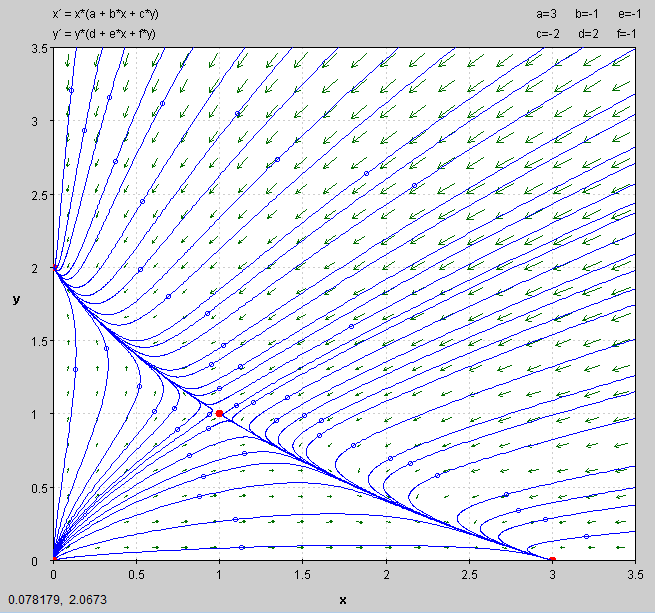
\includegraphics[width = 0.9\textwidth, height = 0.5\textwidth]{-2-1}
  \end{center}
  \caption{Phase portrait of the system in \eqref{eqn:PPSystem}, which has an unstable node at \mbox{(0,0)}, two stable points at \mbox{(0,2)} and \mbox{(3,0)} and a saddle point at \mbox{(1,1)}. All the equilibriums are marked by large dots and selected trajectories are marked by solid lines. This figure was generated using PPLANE (\texttt{http://math.rice.edu/~dfield/dfpp.html}).}
  \label{fig:pplane}
\end{figure*}

\begin{figure*}[p] % The * makes the figure span both columns, p places the figure on a float page
  \begin{center}
    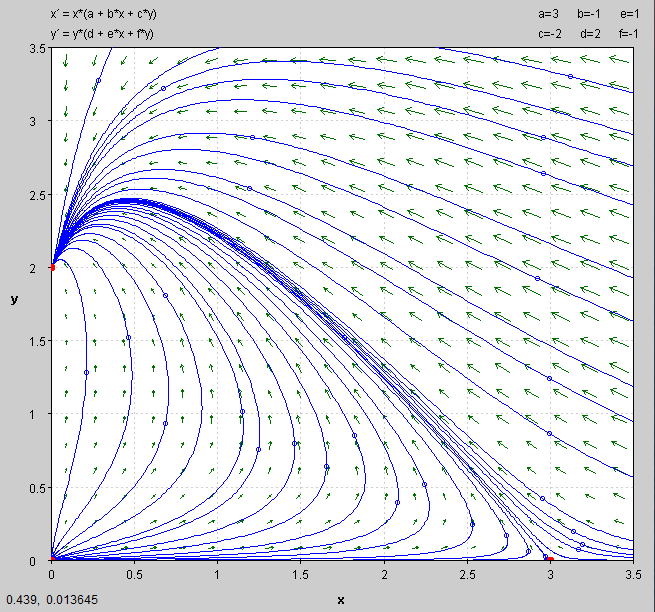
\includegraphics[width = 0.9\textwidth, height = 0.5\textwidth]{-21}
  \end{center}
  \caption{Phase portrait of the system in \eqref{eqn:PPSystem}, which has an unstable node at \mbox{(0,0)}, a stable point at \mbox{(0,2)} and a saddle at \mbox{(3,0)}. All the equilibriums are marked by large dots and selected trajectories are marked by solid lines. This figure was generated using PPLANE (\texttt{http://math.rice.edu/~dfield/dfpp.html}).}
  \label{fig:pplane2}
\end{figure*}

\begin{figure*}[p] % The * makes the figure span both columns, p places the figure on a float page
  \begin{center}
    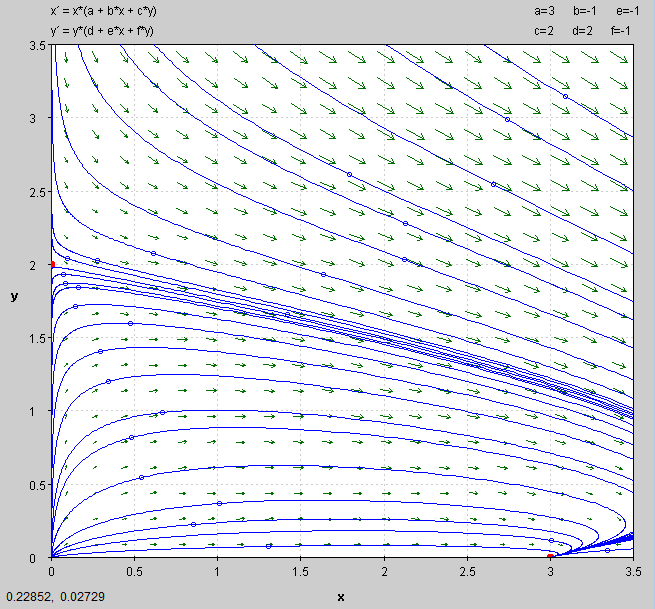
\includegraphics[width = 0.9\textwidth, height = 0.5\textwidth]{2-1}
  \end{center}
  \caption{Phase portrait of the system in \eqref{eqn:PPSystem}, which has an unstable node at \mbox{(0,0)}, a saddle point at \mbox{(0,2)} and a stable at \mbox{(3,0)}. All the equilibriums are marked by large dots and selected trajectories are marked by solid lines. This figure was generated using PPLANE (\texttt{http://math.rice.edu/~dfield/dfpp.html}).}
  \label{fig:pplane2}
\end{figure*}

\begin{figure*}[p] % The * makes the figure span both columns, p places the figure on a float page
  \begin{center}
    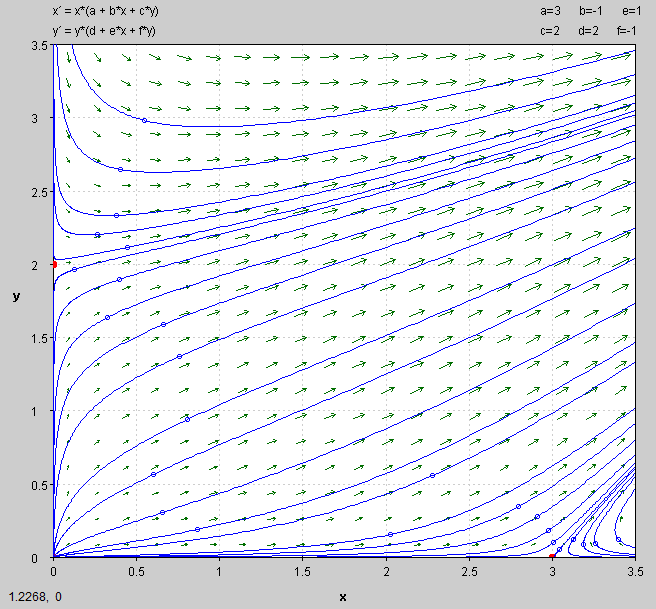
\includegraphics[width = 0.9\textwidth, height = 0.5\textwidth]{21}
  \end{center}
  \caption{Phase portrait of the system in \eqref{eqn:PPSystem}, which has an unstable node at \mbox{(0,0)}, two saddle points at \mbox{(0,2)} \mbox{(3,0)}. All the equilibriums are marked by large dots and selected trajectories are marked by solid lines. This figure was generated using PPLANE (\texttt{http://math.rice.edu/~dfield/dfpp.html}).}
  \label{fig:pplane2}
\end{figure*}

\begin{figure*}[p] % The * makes the figure span both columns, p places the figure on a float page
  \begin{center}
    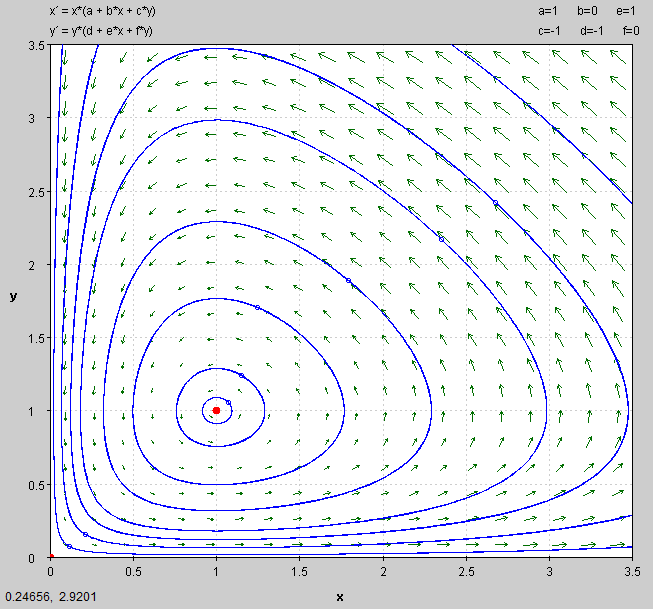
\includegraphics[width = 0.9\textwidth, height = 0.5\textwidth]{p3}
  \end{center}
  \caption{Phase portrait of the system in \eqref{eqn:PPSystem}, which has a saddle node at \mbox{(0,0)} and a stable point at \mbox{(1,1)}. All the equilibriums are marked by large dots and selected trajectories are marked by solid lines. This figure was generated using PPLANE (\texttt{http://math.rice.edu/~dfield/dfpp.html}).}
  \label{fig:pplane2}
\end{figure*}





\end{document}      % End of the document
